\documentclass[10pt,letterpaper]{article}
\usepackage{amsmath}
\usepackage{amsfonts}
\usepackage{amssymb}
\usepackage[utf8]{inputenc}
\usepackage{makeidx}
\usepackage{graphicx}
\usepackage{lmodern}
\usepackage[left=2cm,right=2cm,top=2cm,bottom=2cm]{geometry}
%Used for color for programming language
\usepackage{listings}
\usepackage{color}

\newcommand{\hmwkTitle}{Assignment\ \#1} % Assignment title
\newcommand{\hmwkDueDate}{11:59pm January 28,\ 2018} % Due date
\newcommand{\hmwkClass}{CS 535} % Course/class
\newcommand{\hmwkClassTime}{16:20} % Class/lecture time
\newcommand{\hmwkClassInstructor}{Alexander C. Nwala} % Teacher/lecturer
\newcommand{\hmwkAuthorName}{David Sinclair} % Your name

%----------------------------------------------------------------------------------------
%	TITLE PAGE
%----------------------------------------------------------------------------------------

\title{
\vspace{2in}
\textmd{\textbf{\hmwkClass:\ \hmwkTitle}}\\
\normalsize\vspace{0.1in}\small{Due\ on\ \hmwkDueDate}\\
\vspace{0.1in}\large{\textit{\hmwkClassInstructor\ \hmwkClassTime}}
\vspace{3in}
}
\author{\textbf{\hmwkAuthorName}}


\begin{document}

\maketitle
%----------------------------------------------------------------------------------------
%	TABLE OF CONTENTS
%----------------------------------------------------------------------------------------

%\setcounter{tocdepth}{1} % Uncomment this line if you don't want subsections listed in the ToC

\pagebreak
\tableofcontents
\pagebreak 

%----------------------------------------------------------------------------------------
%	Create colors for scripting 
%----------------------------------------------------------------------------------------


\definecolor{dkgreen}{rgb}{0,0.6,0}
\definecolor{gray}{rgb}{0.5,0.5,0.5}
\definecolor{mauve}{rgb}{0.58,0,0.82}

\lstset{frame=tb,
  language=Python,
  aboveskip=3mm,
  belowskip=3mm,
  showstringspaces=false,
  columns=flexible,
  basicstyle={\small\ttfamily},
  numbers=none,
  numberstyle=\tiny\color{gray},
  keywordstyle=\color{blue},
  commentstyle=\color{dkgreen},
  stringstyle=\color{mauve},
  breaklines=true,
  breakatwhitespace=true,
  tabsize=3
}
%----------------------------------------------------------------------------------------
%	Problem 1 %----------------------------------------------------------------------------------------

\section{Problem 1}
\subsection{Question 1}
Demonstrate that you know how to use "curl" well enough to correctly POST data to a form.  Show that the HTML response that is returned is "correct".  That is, the server should take the arguments you POSTed and build a response accordingly.  Save the HTML response to a file and then view that file in a browser and take a screen shot.
\subsection{Answer 1}
I used curl and submitted the following into the terminal.
\\
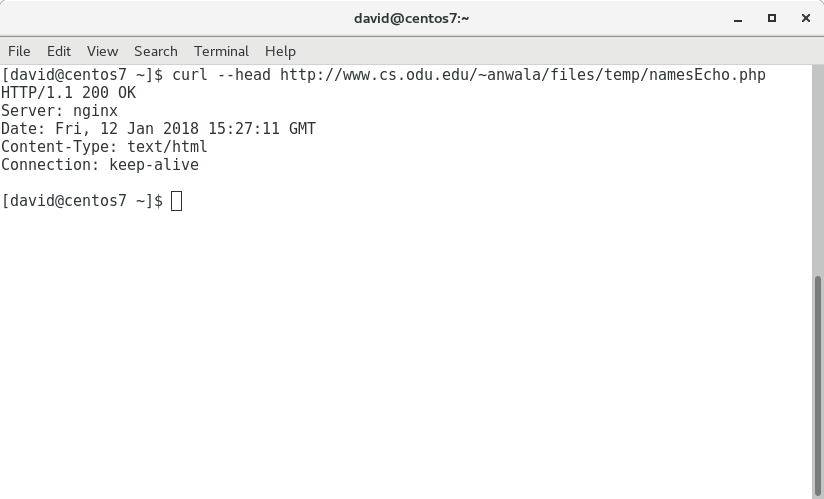
\includegraphics[scale=.25]{curl_head.png}
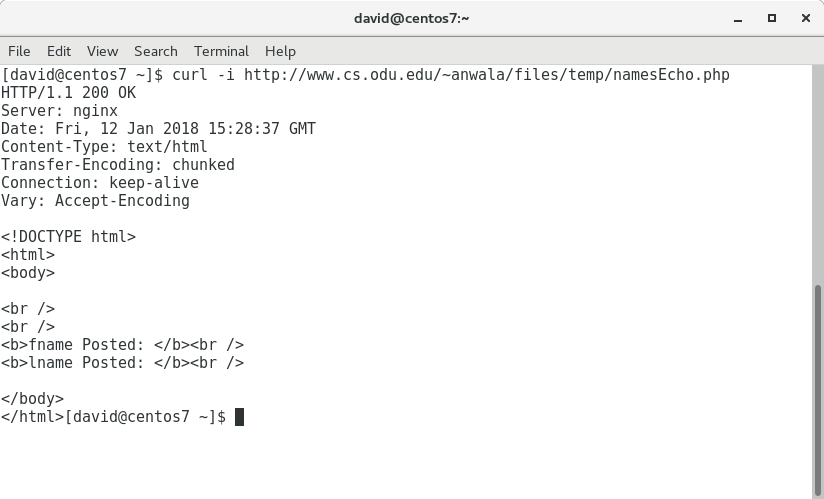
\includegraphics[scale=.25]{curl_i.png}
\\
After I used curl to determine the naming required to input or POST on the web page.  I added the following curl command\\
\\
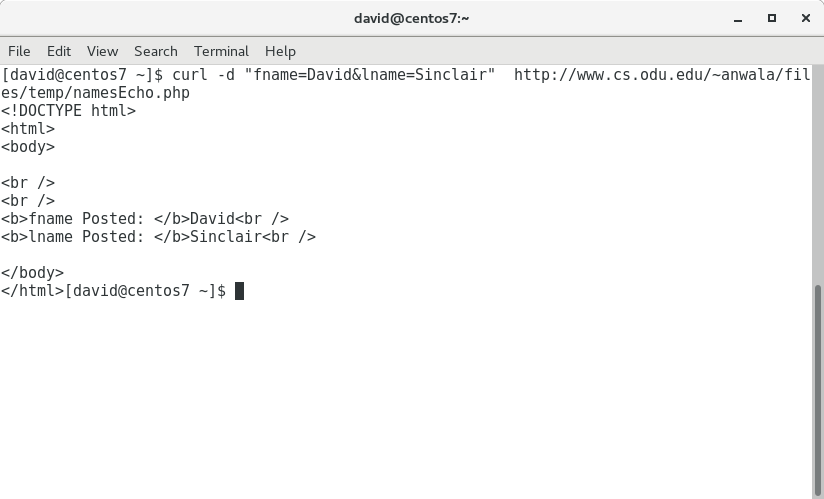
\includegraphics[scale=.25]{curl_results.png} 

\pagebreak % Create Page break between problems

%----------------------------------------------------------------------------------------
%	Problem 2
%----------------------------------------------------------------------------------------

\section{Problem 2}
\subsection{Question 2}
2.  Write a Python program that:\\
  1. takes as a command line argument a web page\\
  2. extracts all the links from the page\\
  3. lists all the links that result in PDF files, and prints out the bytes for each of the links.  (note: be sure to follow all the redirects until the link terminates with a "200 OK".)\\
  4. show that the program works on 3 different URIs, one of which needs to be:\\
     http://www.cs.odu.edu/~mln/teaching/cs532-s17/test/pdfs.html

\subsection{Answer 2}
The program is called problem2.py.  To use the program it is written with python3.  The following libraries for python 3 will be needed:\\
\\
1. Beautiful Soup\\
2. urlopen\\
3. validartors\\
4. requests\\
\\
Without these libraries this program will fail.\\
\\
To meet requirement 1 of question 2.  I used the following code:\\
This takes the arguments from the command line and prints them.
\begin{lstlisting}
#LIST the ARGUMENTS used to start this program
print("This is the name of the script: ", sys.argv[0])
print("Number of arguments: ", len(sys.argv))
print("The arguments are: ", str(sys.argv))

if len(sys.argv) == 2:
        url = sys.argv[1]
        print(url)
else:
	print("Wrong number of arguments!")
	print("Usage: python3 problem2.py http://<URL>")
	sys.exit()
\end{lstlisting}
To meet requirement 2 of question 2. I used the following code:\\
This takes the 2nd argument, which is a url address.  Gets the html of the page and removes the links from it and appends it to an array.
\cite{bsdoc_2015}
\cite{digitalocean_2017}
\begin{lstlisting}
#Sets the webpage and open
#url = "http://www.cs.odu.edu/~mln/teaching/cs532-s17/test/pdfs.html" 
html_page = urlopen(url)
#parses the webpage 
soup = BeautifulSoup(html_page, "html.parser")

#Creates the array for adding links to
links = []

#Parses the webpage and pulls out all the links
for link in soup.findAll('a', attrs={'href': re.compile("^http")}):
#	print(link.get('href'))
	links.append(link.get('href'))
\end{lstlisting}
To meet requirement 3 of question 2. I used the following code:\\
This takes the array created in requirement 2 and removes the pdf links.  The code then gets the header for the pdf links and gets the content length.  It then prints out the results.
\cite{stackoverflow}
\begin{lstlisting}
#Prints the number of links and Counts the number of links
print("\nThe number of URL's is ",len(links),"\n")  
print(*links,sep='\n')
#looks at the links files and removes all the .pdf files into a new aray.
matching = [s for s in links if ".pdf" in s]
print("\nThere is ",len(matching)," pdf files on the ",url,"webpage.\n")

print(*matching,sep='\n')

for index , url2 in enumerate(matching):
#I want to open the URL listed in my list, get the header and print the content-legth
	resp = requests.get(url2)
	print(url2,"has a file size of ",resp.headers['content-length'],"bytes.\n")
\end{lstlisting}
To meet requirement 4 of question 2. I attached the following screen shots:\\
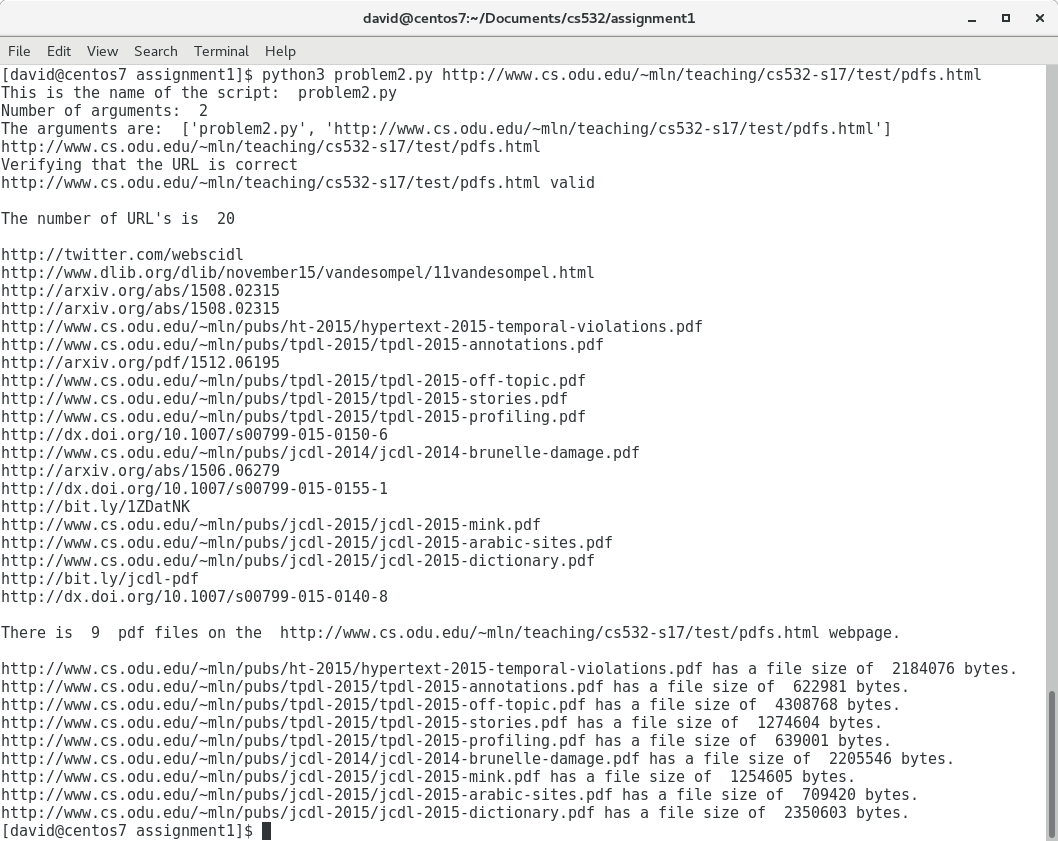
\includegraphics[scale=.25]{problem2req4a.png}
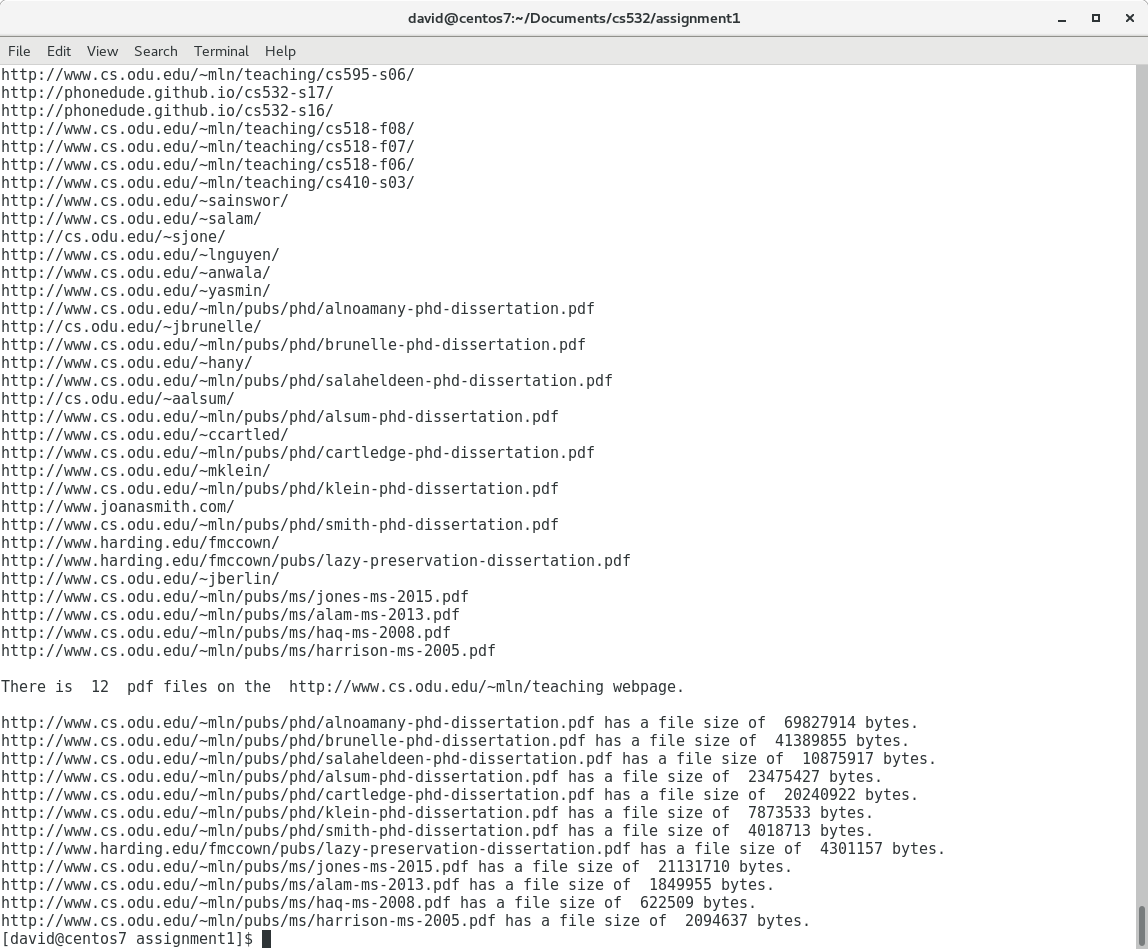
\includegraphics[scale=.25]{problem2req4c.png}
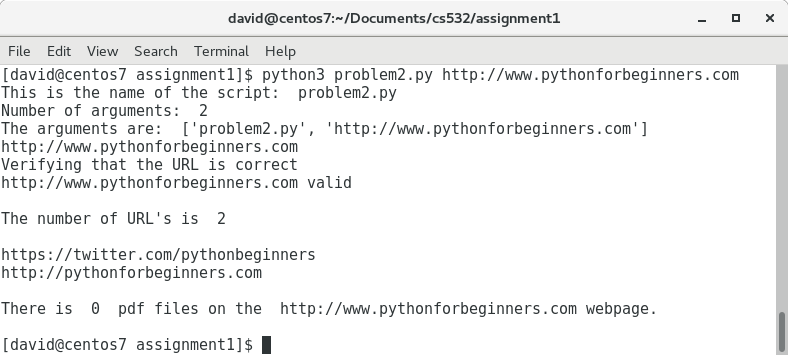
\includegraphics[scale=.25]{problem2req4b.png}

\pagebreak% Create Page break between problems

%----------------------------------------------------------------------------------------
%	Problem 3
%----------------------------------------------------------------------------------------

\section{Problem 3}
\subsection{Question 3}
3.  Consider the "bow-tie" graph in the Broder et al. paper (fig 9):\\ 
    http://www9.org/9cdrom/160/160.html\\ 
\\ 
    Now consider the following graph:\\ 
\\ 
    A --$>$ B\\ 
    B --$>$ C\\ 
    C --$>$ D\\ 
    C --$>$ A\\ 
    C --$>$ G\\ 
    E --$>$ F\\ 
    G --$>$ C\\ 
    G --$>$ H\\ 
    I --$>$ H\\ 
    I --$>$ K\\ 
    L --$>$ D\\
    M --$>$ A\\ 
    M --$>$ N\\ 
    N --$>$ D\\ 
    O --$>$ A\\ 
    P --$>$ G\\ 
\\
    For the above graph, give the values for:\\ 
\\
    IN:\\ 
    SCC:\\ 
    OUT:\\ 
    Tendrils:\\
    Tubes:\\ 
    Disconnected:\\ 
\\ 
\subsection{Answer 3}
\begin{lstlisting}
import matplotlib.pyplot as plt
import numpy as np


def add_arrow(line, position=None, direction='right', size=15, color=None):
    """
    add an arrow to a line.

    line:       Line2D object
    position:   x-position of the arrow. If None, mean of xdata is taken
    direction:  'left' or 'right'
    size:       size of the arrow in fontsize points
    color:      if None, line color is taken.
    """
    if color is None:
        color = line.get_color()

    xdata = line.get_xdata()
    ydata = line.get_ydata()

    if position is None:
        position = xdata.mean()
    # find closest index
    start_ind = np.argmin(np.absolute(xdata - position))
    if direction == 'right':
        end_ind = start_ind + 1
    else:
        end_ind = start_ind - 1

    line.axes.annotate('',
        xytext=(xdata[start_ind], ydata[start_ind]),
        xy=(xdata[end_ind], ydata[end_ind]),
        arrowprops=dict(arrowstyle="->", color=color),
        size=size
    )


n=['A','B','C','D','E','F','G','H','I','J','K','L','M','N','O','P'] 
a=[ 2 , 3 , 4 , 7 , 5 , 6 , 4 , 7 , 0 , 0 , 1 , 0 , 2 , 4 , 0 , 0]
b=[ 3 , 2 , 2,  2,  0 , 0 , 3 , 3 , 5 , 0,  5,  1,  2 , 1 , 2 , 3]

fig, ax = plt.subplots()
ax.scatter(a, b)



for i, txt in enumerate(n):
    ax.annotate(txt, (a[i],b[i]))

#ax = plt.axes()
#ax.arrow(1, 1, 0, 1, head_width=0.05, head_length=0.1, fc='k', ec='k')
#plt.show()

#    A --> B 
x= [2,3]
y= [3,2]
plt.plot(x,y, label="A --> B")[0]
#  B --> C
x2 = [3,4]
y2 = [2,2]
plt.plot(x2, y2, label="B --> C")[0]
#    C --> D
x3 = [4,7]
y3 = [2,2]
plt.plot(x3, y3, label="C --> D")
#    C --> A  
x4 = [4,2]
y4 = [2,3]
plt.plot(x4, y4, label="C --> A")
#    C --> G
x5 = [4,4]
y5 = [2,3]
plt.plot(x5, y5, label="C --> G")
#    E --> F
x6 = [5,6]
y6 = [0,0]
plt.plot(x6, y6, label="E --> F")
#    G --> C
x7 = [4,4]
y7 = [3,2]
plt.plot(x7, y7, label="G --> C")
#    G --> H
x8 = [4,7]
y8 = [3,3]
plt.plot(x8, y8, label="G --> H")
#    I --> H
x9 = [0,7]
y9 = [5,3]
plt.plot(x9, y9, label="I --> H")
#    I --> K
x10 = [0,1]
y10 = [5,5]
plt.plot(x10, y10, label="I --> K")
#    L --> D
x11 = [0,7]
y11 = [1,2]
plt.plot(x11, y11, label="L --> D")
#    M --> A
x12 = [2,2]
y12 = [2,3]
plt.plot(x12, y12, label="M --> A")
#    M --> N
x13 = [2,4]
y13 = [2,1]
plt.plot(x13, y13, label="M --> N")
#    N --> D
x14 = [4,7]
y14 = [1,2]
plt.plot(x14, y14, label="N --> D")
#    O --> A
x15 = [0,2]
y15 = [2,3]
plt.plot(x15, y15, label="O --> A")
#    P --> G 
x16 = [0,4]
y16 = [3,3]
plt.plot(x16, y16, label="P --> G")

plt.xlabel('Plot Number')
plt.ylabel('Important var')
plt.title('Determining Bow Tie for Points')
plt.legend()
plt.show()
\end{lstlisting}
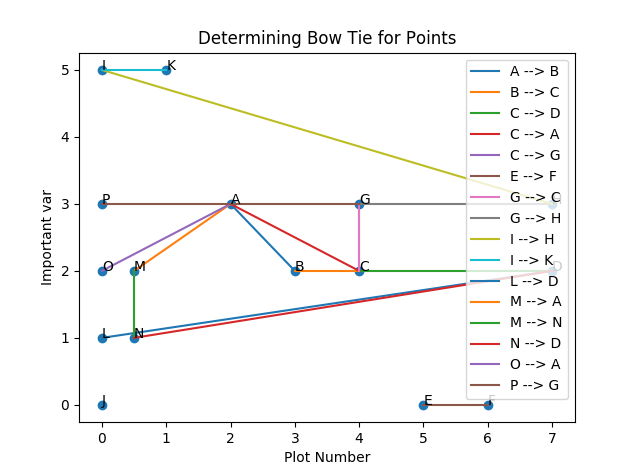
\includegraphics[scale=.5]{Figure_1.png} 
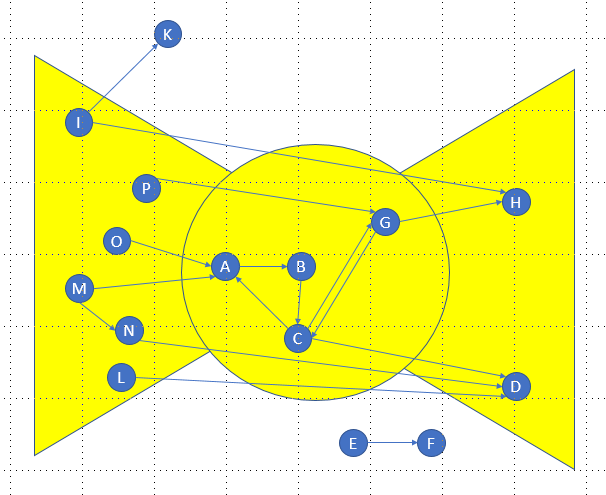
\includegraphics[scale=.4]{question3.png} 
\\
\\
I then compared to the Bow Tie points.\\
\\
From the comparison using the below as the criteria.\\
    1. IN: Pages with no in-links or in-links from IN pages and out-links to pages in IN, SCC, Tendrils, or Tubes.\\ 
    2. SCC: Pages with in-links from IN or SCC and out-links to OUT or SCC. There exists some path of links from every page in SCC to every other page in SCC.\\
    3. OUT: Pages with no out-links or out-links to other pages in OUT, and all in-links come from OUT, SCC, Tendrils, or Tubes.\\ 
    4. Tendrils: Pages that can only be reached from IN or have only out-links to OUT. \\
    5. Tubes: Pages that have in-links from IN or other pages in Tubes and out-links to pages in Tubes or OUT.\\ 
    6. Disconnected: Pages that have no in-links from any other components and no out-links to other components. These pages may be linked to each other.\\
\cite{broder_2003}
\\
I believe that:\\
    IN: I, L, O, P\\ 
    SCC:A, B, C, G, M, N\\ 
    OUT:D, H \\ 
    Tendrils:I-K\\
    Tubes: L-D \\ 
    Disconnected:E-F\\ 

\pagebreak% Create Page break between problems

\bibliographystyle{plain}
\bibliography{mylib}

\end{document}